\section{A PDE optimal control problem}
NY:
We have some physical one-dimensional object, $\Omega = (0, 1)$, that we wish to give a desired temperature profile $y_d \in L^2 (\Omega)$.
The boundaries of the object are set to a (relative) temperature of $0$. 
There is some heat source $u$ that we have control over, but there is a cost $\alpha \in (0, \infty)$ associated with both cooling and heating the object.

GAMMEL:
A physical object $\Omega = (0, 1)$ is to be heated or cooled to some desired temperature profile $y_d \in L^2 (\Omega)$. The (relative) temperature is $0$ at the boundaries. 
We can control a heat source $u$ and there is some cost $\alpha \in (0, \infty)$ associated with heating/cooling the object.


Our problem is then to minimize the discrepancy between the desired profile and the temperature profile of the object, while simultaneously minimizing the cost of the heating/cooling.
Our problem then becomes
\begin{equation}
    \label{eq:OCP}
    \min_{y, u} \frac{1}{2} \int_0^1 \lvert y - y_d \rvert^2 dx + \frac{\alpha}{2}\int_0^1u^2 dx
    \quad \text{s.t.} \quad \begin{cases}
       -\Delta y = u \\
       y(0) = y(1) = 0
    \end{cases} 
    \quad \text{in the weak sense.}
\end{equation}
We approximate this as 
\begin{equation}
    \label{eq:OCP_FE}
    \min_{u_h, y_h \in V_h} \frac{1}{2} \lVert y_h - \bar{y_d} \rVert_ {L^2(\Omega)}^2 + \frac{\alpha}{2} \lVert u_h \rVert_{L^2(\Omega)}^2
    \quad \text{s.t.} \quad a(y_h, v) = \langle u_h, v \rangle_{L^2(\Omega)} \forall v \in V_h,
\end{equation}
where $\bar{y}_d$ is the interpolation of $y_d$ onto $X_h^2$, $V_h = X_h^2 \cap H_0^1 (\Omega)$ and $a(u, v) = \int_0^1 u_x v_x dx$.
The optimal control is then $u_h$, and the optimal state is $y_h$.


\subsection{Solution}
To find a solution we interpret this as a minimization problem for the unknown coefficients $\mathbf{u} = \{u_1, \dots, u_{2N-1} \}$, $\mathbf{y} = \{y_1, \dots, y_{2N-1} \}$ as
\begin{equation}
    \label{eq:OCP_coeff}
    \min_{\mathbf{y,u} \in \mathds{R}^{2N-1}} G(\mathbf{y, u}) \quad \text{s.t.} \quad B\mathbf{y} = F\mathbf{u}.
\end{equation}
For $F$ and $B$ we use each side of the constraint from (\ref{eq:OCP_FE}), 
\begin{align*}
    a(y_h, v) &= \int_0^1 \left( \sum_{i=1}^{2N-1} y_i \varphi_i'  \right) \left( \sum_{j=1}^{2N-1} v_j \varphi_j'\right)dx  \\
    & = \sum_{i=1}^{2N-1}\sum_{j=1}^{2N-1} y_i v_j\int_0^1  \varphi_i' \varphi_j' dx \\
    &= \mathbf{v}^T B \mathbf{y} ,
\end{align*}
where $B_{i,j} = \int_0^1 \varphi_i' \varphi_j'dx$,  $i,j = 1, \dots, 2N-1$, which is the stiffness matrix, and  
\begin{align*}
    \langle u_h, v \rangle_{L^2(\Omega)} &= \int_0^1 \left( \sum_{i=1}^{2N-1} u_i \varphi_i \right) \left( \sum_{j=1}^{2N-1} v_j \varphi_j \right) dx \\
    &= \sum_{i=1}^{2N-1}\sum_{j=1}^{2N-1} u_i v_j\int_0^1  \varphi_i \varphi_j dx \\
    &= \mathbf{v}^T F \mathbf{u} , 
\end{align*}
 where $F_{i,j}=\int_0^1  \varphi_i \varphi_j dx$, $i,j = 1, \dots, 2N-1$.
Hence \( \mathbf{v}^T B \mathbf{y} = \mathbf{v}^T F \mathbf{u}  \) and
since the constraint holds for all $\mathbf{v} \in V_h$, we get that
$$B\mathbf{y} = F \mathbf{u}.$$

We find $G(\mathbf{y, u})$ by rewriting the objective function of (\ref{eq:OCP_FE}).
Since the desired profile is an interpolation, we know that $\bar{y}_d = \sum_{i=0}^{2N}d_i\varphi_i$,
where $\mathbf{d} = \begin{bmatrix} d_0 & \dots & d_{2N} \\ \end{bmatrix}^T$
are the coefficients,
giving the form
\begin{align*}
    G(\mathbf{y, u}) &= \frac{1}{2}\langle y_h - \bar{y}_d, y_h - \bar{y}_d \rangle_{L^2{(\Omega)}} + \frac{\alpha}{2} \langle u_h, u_h \rangle_{L^2(\Omega)} \\
   &= \frac{1}{2}\langle y_h , y_h \rangle_{L^2{(\Omega)}} +  \frac{1}{2}\langle \bar{y}_d ,\bar{y}_d  \rangle_{L^2{(\Omega)}}
   - \langle y_h, \bar{y}_d \rangle_{L^2{(\Omega)}} + \frac{\alpha}{2} \langle u_h, u_h \rangle_{L^2(\Omega)} \\
     &= \frac{1}{2}\int_0^1\left( \sum_{i=1}^{2N-1}y_i \varphi_i \right)^2dx  + \frac{1}{2}\int_0^1\left( \sum_{i=0}^{2N}d_i \varphi_i \right)^2dx \\
     &\quad- \int_0^1\left( \sum_{i=1}^{2N-1}y_i \varphi_i \right) \left(\sum_{i=0}^{2N} d_i \varphi_i \right)dx + 
     \frac{\alpha}{2}\int_0^1\left(\sum_{i=1}^{2N-1} u_i \varphi_i  \right)^2dx \\    
     &= \frac{1}{2}\sum_{i=1}^{2N-1}\sum_{j=1}^{2N-1} y_i y_j \int_0^1 \varphi_i \varphi_j dx + \frac{1}{2}\sum_{i=0}^{2N}\sum_{j=0}^{2N} d_i d_j \int_0^1 \varphi_i \varphi_j dx \\
    &\quad- \sum_{i=1}^{2N-1} \sum_{j=0}^{2N} y_i d_i \int_0^1 \varphi_i \varphi_j dx +  \frac{\alpha}{2}\sum_{i=1}^{2N-1}\sum_{j=1}^{2N-1} u_i u_j \int_0^1\varphi_i \varphi_j dx.
\end{align*}
We can rewrite this in the form
$$
G(\mathbf{y, u}) = \frac{1}{2}\mathbf{y}^T F \mathbf{y} + \frac{1}{2}\mathbf{d}^T\Tilde{F} \mathbf{d} - \mathbf{y}^T\hat{F}\mathbf{d} + \frac{\alpha}{2}\mathbf{u}^T F \mathbf{u},
$$
where $\Tilde{F} \in \mathds{R}^{(2N+1) \times (2N+1)}$
is $F$, but extended to include the boundaries.
$\hat{F} \in \mathds{R}^{(2N-1) \times (2N+1)}$ is the same as $\Tilde{F}$ but with the first and last row removed.  

To solve equation (\ref{eq:OCP_coeff}) we use Lagrange multipliers and the Lagrangian
\begin{align}
    \label{eq:OCP_lagrangian}
    \mathcal{L}(\mathbf{y, u, \lambda}) &= G(\mathbf{y, u}) - \mathbf{\lambda}^T \left( B\mathbf{y} - F\mathbf{u} \right) \\
    &= \frac{1}{2}\mathbf{y}^T F \mathbf{y} + \frac{1}{2}\mathbf{d}^T\Tilde{F} \mathbf{d} - \mathbf{y}^T\hat{F}\mathbf{d} + \frac{\alpha}{2}\mathbf{u}^T F \mathbf{u}  - \mathbf{\lambda}^T \left( B\mathbf{y} - F\mathbf{u} \right) ,
\end{align}
where $\mathbf{\lambda} \in \mathds{R}^{2N-1}$ is the vector of Lagrange multipliers.
The solution is found by solving
\begin{align}
    \label{eq:gradients}
    \nabla_{\mathbf{y}}\mathcal{L} = 0 \\
    \nabla_{\mathbf{u}}\mathcal{L} = 0 \\
    \nabla_{\mathbf{\mathbf{\lambda}}}\mathcal{L} = 0
\end{align}
for $\mathbf{y}$ and $\mathbf{u}$.
Calculating the gradients, and exploiting the symmetry of \( F \) and \( B \)
yields the system
\begin{align}
  F \mathbf{y}- \hat{F}\mathbf{d} - B\mathbf{\lambda} &= 0 \\
  \alpha F \mathbf{u}+ F\mathbf{\lambda} &= 0 \\
  -B \mathbf{y} + F \mathbf{y} &= 0
\end{align}

\begin{lemma}
    $F$ is positive definite.    
\end{lemma}
\begin{proof}
    \label{lemma:F_invertible}
    The basis functions $\varphi_i$ are linearly independent, since they are Lagrange nodal polynomials and our nodes are unique.
    Since $F_{i,j} = \int_0^1 \varphi_i \varphi_j dx = \langle \varphi_i, \varphi_j \rangle_{L^2(\Omega)}$,
    $F$ is a Gram-matrix corresponding to the vector space of our basis functions.
    Combining these results gives us that $F$ is positive definite.
\end{proof}

\begin{lemma}
    \label{lemma:B_pos_def}
    $B$ is positive definite.
\end{lemma}
\begin{proof}
    Let $\mathbf{z} \in \mathds{R}^{(2N-1)}$, then 
    $$\mathbf{z}^T B \mathbf{z} = \sum_{i=1}^{2N-1}\sum_{j=1}^{2N-1} z_i B_{i,j}z_j =\sum_{i=1}^{2N-1}\sum_{j=1}^{2N-1}a(v_i \varphi_i, v_j\varphi_j) >0 .$$
\end{proof}

\begin{lemma}
    $BF^{-1}B$ is positive definite.
\end{lemma}
\begin{proof}
    $F^{-1}$ is positive definite since it is the inverse of a positive definite matrix and $\ker(B) = \{0\}$ since $B$ is positive definite, by lemma (\ref{lemma:B_pos_def}).
    
    Let $\mathbf{z} \in \mathds{R}^{2N-1}$,
    $$\mathbf{z}^T BF^{-1}B \mathbf{z} = (B\mathbf{z})^T F^{-1}(B\mathbf{z}) > 0.$$
\end{proof}
Since $F$ is invertible, by lemma (\ref{lemma:F_invertible}), we see that $\alpha \mathbf{u}= -\mathbf{\lambda}$. 
This gives the system
\begin{align}
    \label{eq:lagrange_conditions}
     F \mathbf{y} + \alpha B \mathbf{u} &= \hat{F}\mathbf{d} \\
    -B \mathbf{y} + F \mathbf{u} &= \mathbf{0}.
\end{align}
An explicit solution can be found by seeing that $\mathbf{u}=F^{-1}B \mathbf{y}$, and getting
$$ F\mathbf{y} + \alpha B F^{-1}B \mathbf{y} = \hat{F}\mathbf{d},$$
which gives the solutions
\begin{align*}
    \mathbf{y} &= \left[F + \alpha B F^{-1}B \right]^{-1} \hat{F}\mathbf{d} \\
    \mathbf{u} &= F^{-1} B \left[F + \alpha B F^{-1}B \right]^{-1} \hat{F}\mathbf{d},
\end{align*}
where $\left[F + \alpha B F^{-1}B \right]^{-1}$ exists since $\alpha > 0$ and it is therefore the inverse of the sum of positive definite matrices.
The system can also be written in block matrix form as
$$
\begin{bmatrix}
   F & \alpha B \\
   -B & F \\
\end{bmatrix}
\begin{bmatrix}
    \mathbf{y} \\
    \mathbf{u}
\end{bmatrix}
= 
\begin{bmatrix} \hat{F}\mathbf{d} \\
    \mathbf{0}
\end{bmatrix}.
$$

This system has sparse sub-blocks, which is solved
efficiently by a sparse solver.

\subsection{Example temperature profiles}
We wish to test our implementation for some different desired temperature profiles,
\begin{align}
    y_d &= \frac{1}{2}x(1-x), \label{eq:des_1} \\
    y_d &= 1, \label{eq:des_2}\\
    y_d &= \begin{cases}
        1 \quad \text{for} \quad x \in \left[ \frac{1}{4}, \frac{3}{4}\right] \\
        0 \quad \text{else}.
    \end{cases} \label{eq:des_3}
\end{align}

We see that when the cost parameter is large (\( \alpha = 10^{-1} \), figure \ref{fig:0})
the discrepancy between the optimal state and the
desired profile is quite large.
However, the heating is kept relatively small
(especially compared with figures \ref{fig:1} and \ref{fig:2}).
That is, the optimal control becomes small at the
expense of the discrepancy.

In contrast, for lower costs (\( \alpha = 10^{-8} \),
figure \ref{fig:2}), the discrepancy between the optimal state
and the desired profile is small. 
Note that the distributed heat source reaches amplitudes in
the interval \( (-1500,2000) \) for equations \eqref{eq:des_2} and \eqref{eq:des_3}.

Using a typical cost parameter (\( \alpha = 10^{-3} \), figure \ref{fig:1}),
we see that there is some discrepancy from the
desired profile. The heating profile is reasonable.

This is to be expected given the original problem.
If heating is expensive, the temperature discrepancy is large.
If heating is cheap, the temperature discrepancy is small.

We have assumed that the optimal state, \( y \), and optimal control, \( u \),
are in $H_0^1$, whilst the desired profile, \( y_d \),
are not restricted by \( H_0^1 \).
We get interesting results if we use a desired profile not in $H_0^1$.

This is the case for equations \eqref{eq:des_2} and \eqref{eq:des_3}.
We see that for both high and typical costs,
both the optimal control and state are smooth.

In contrast, for low costs, the optimal control
is rather extreme at the boundaries and at
the discontinuities. TODO: Why?

\begin{figure}
  \centering
  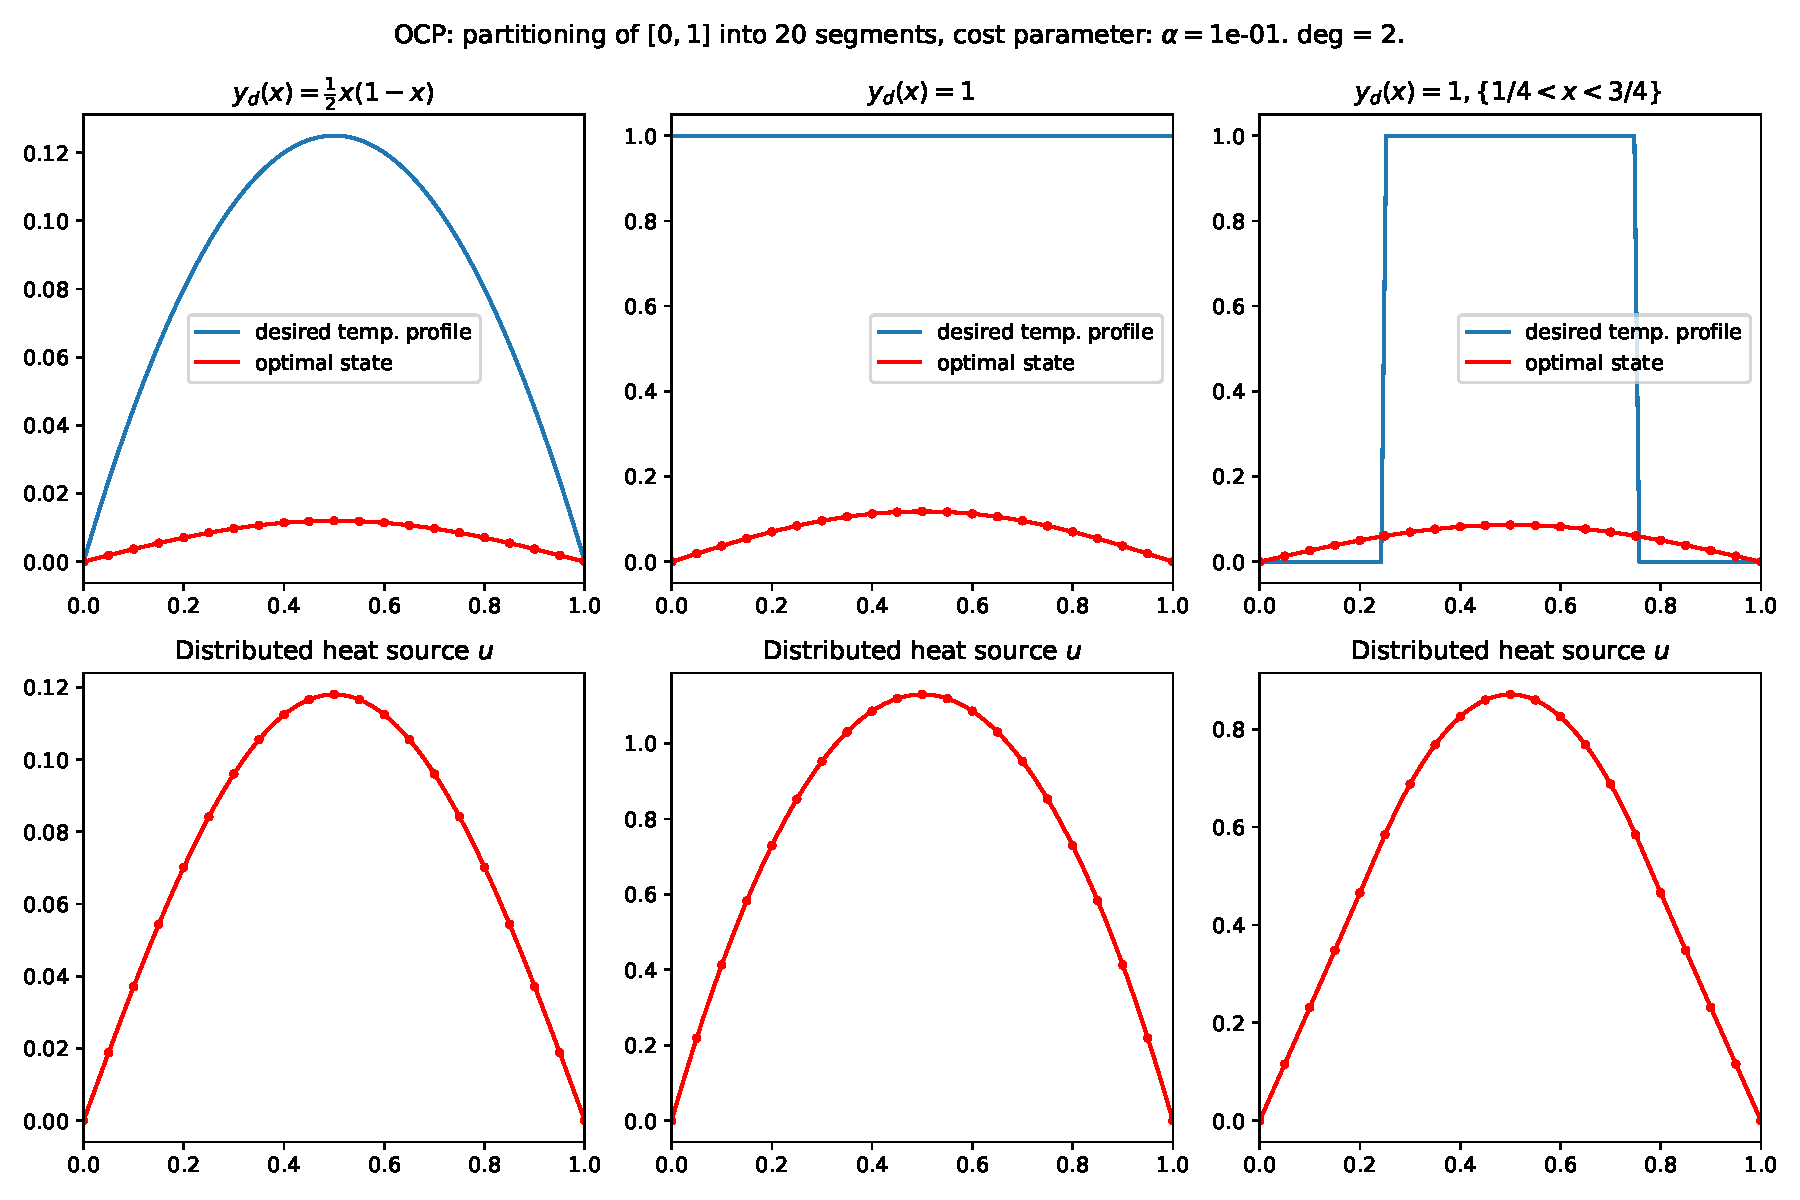
\includegraphics[width=\textwidth]{Images/plots/task2_fig_0.pdf}
  \caption{An optimized control problem for various
    desired temperature profiles. The upper row plots the
    desired temperature profiles and the corresponding 
    optimal state. The lower row plots the
    optimal state for the corresponding problem.
    The cost parameter, $\alpha$, is set to high value.
    To find the optimal state and the optimal control we 
    have partitioned the interval into \( 20 \) elements.
    A second degree Lagrange finite element space has been used.}
  \label{fig:0}
\end{figure}

\begin{figure}
  \centering
  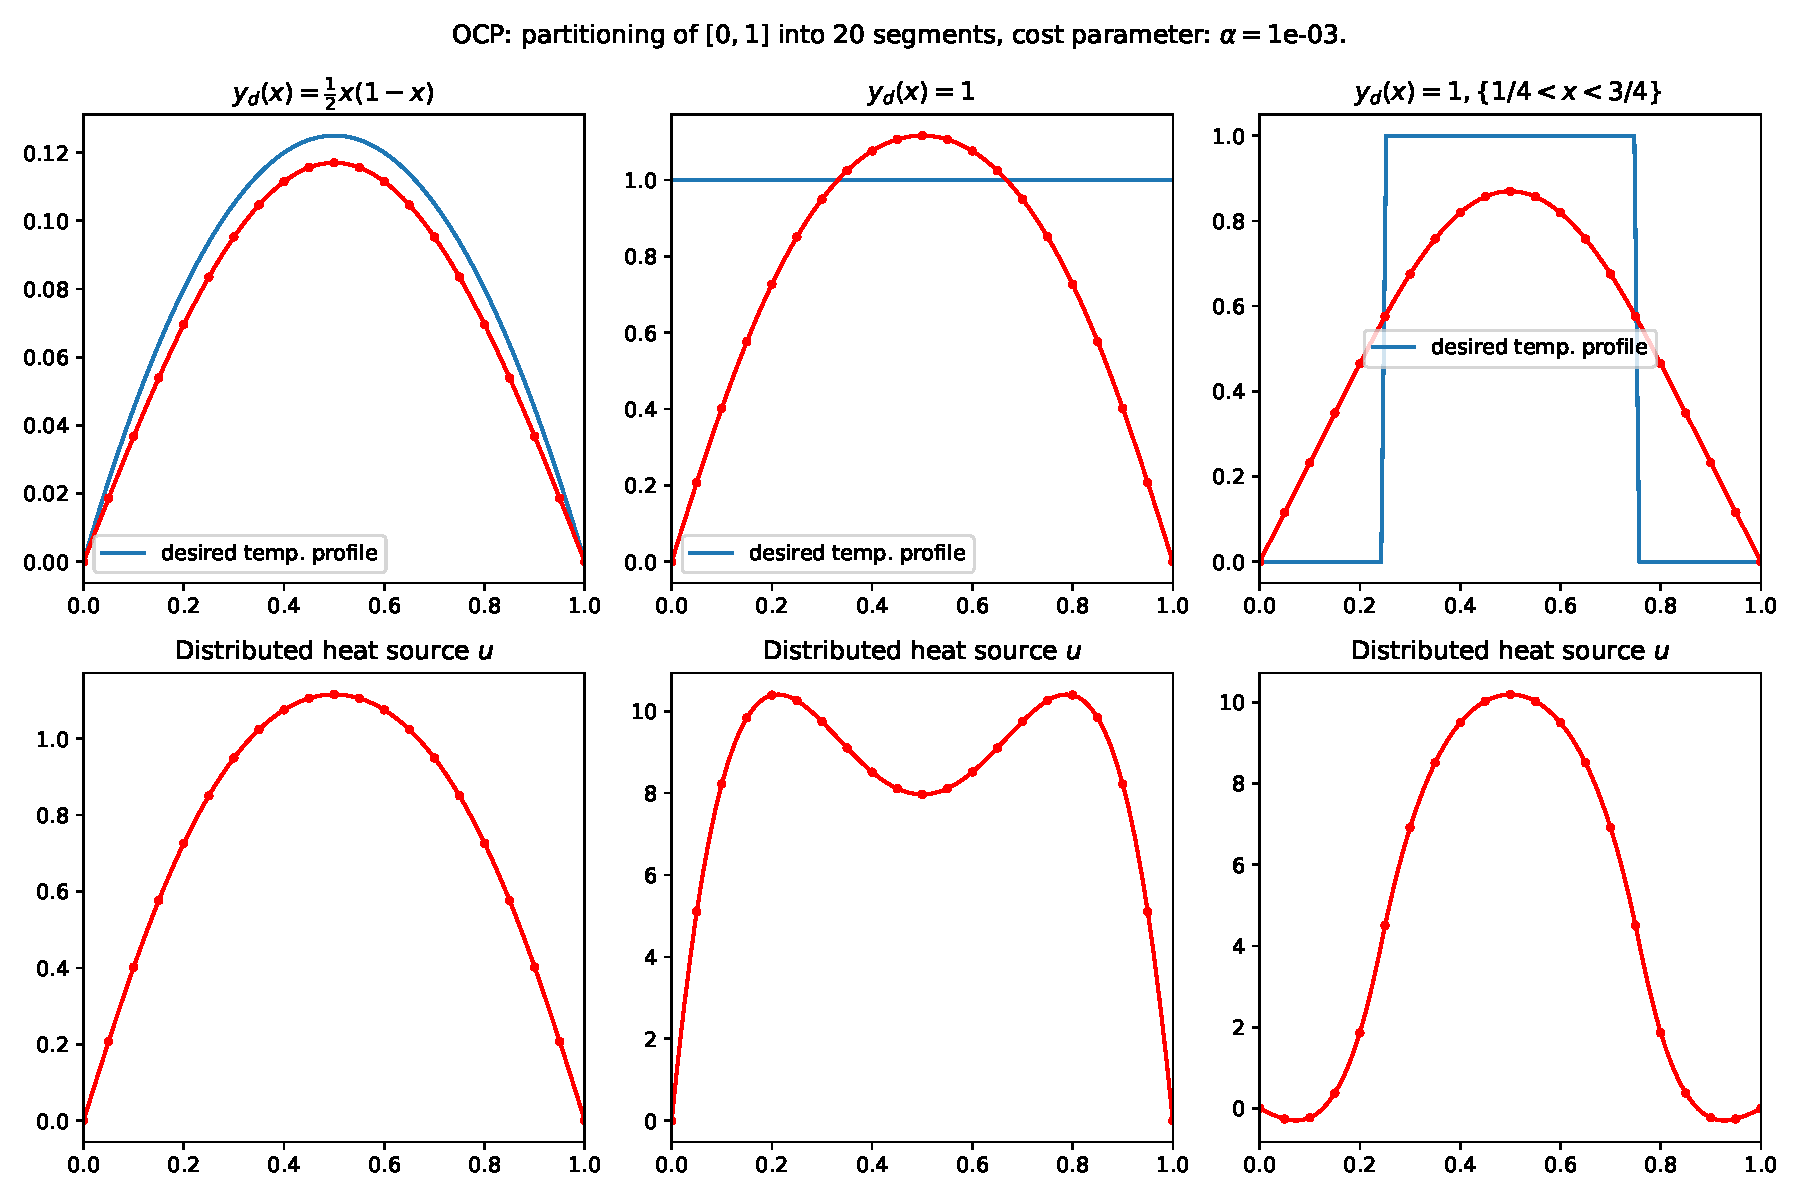
\includegraphics[width=\textwidth]{Images/plots/task2_fig_1.pdf}
  \caption{An optimized control problem for various
    desired temperature profiles. The upper row plots the
    desired temperature profiles and the corresponding 
    optimal state. The lower row plots the
    optimal state for the corresponding problem.
    The cost parameter, $\alpha$, is set to typical value.
    To find the optimal state and the optimal control we 
    have partitioned the interval into \( 20 \) elements.
    A second degree Lagrange finite element space has been used.}
  \label{fig:1}
\end{figure}

\begin{figure}
  \centering
  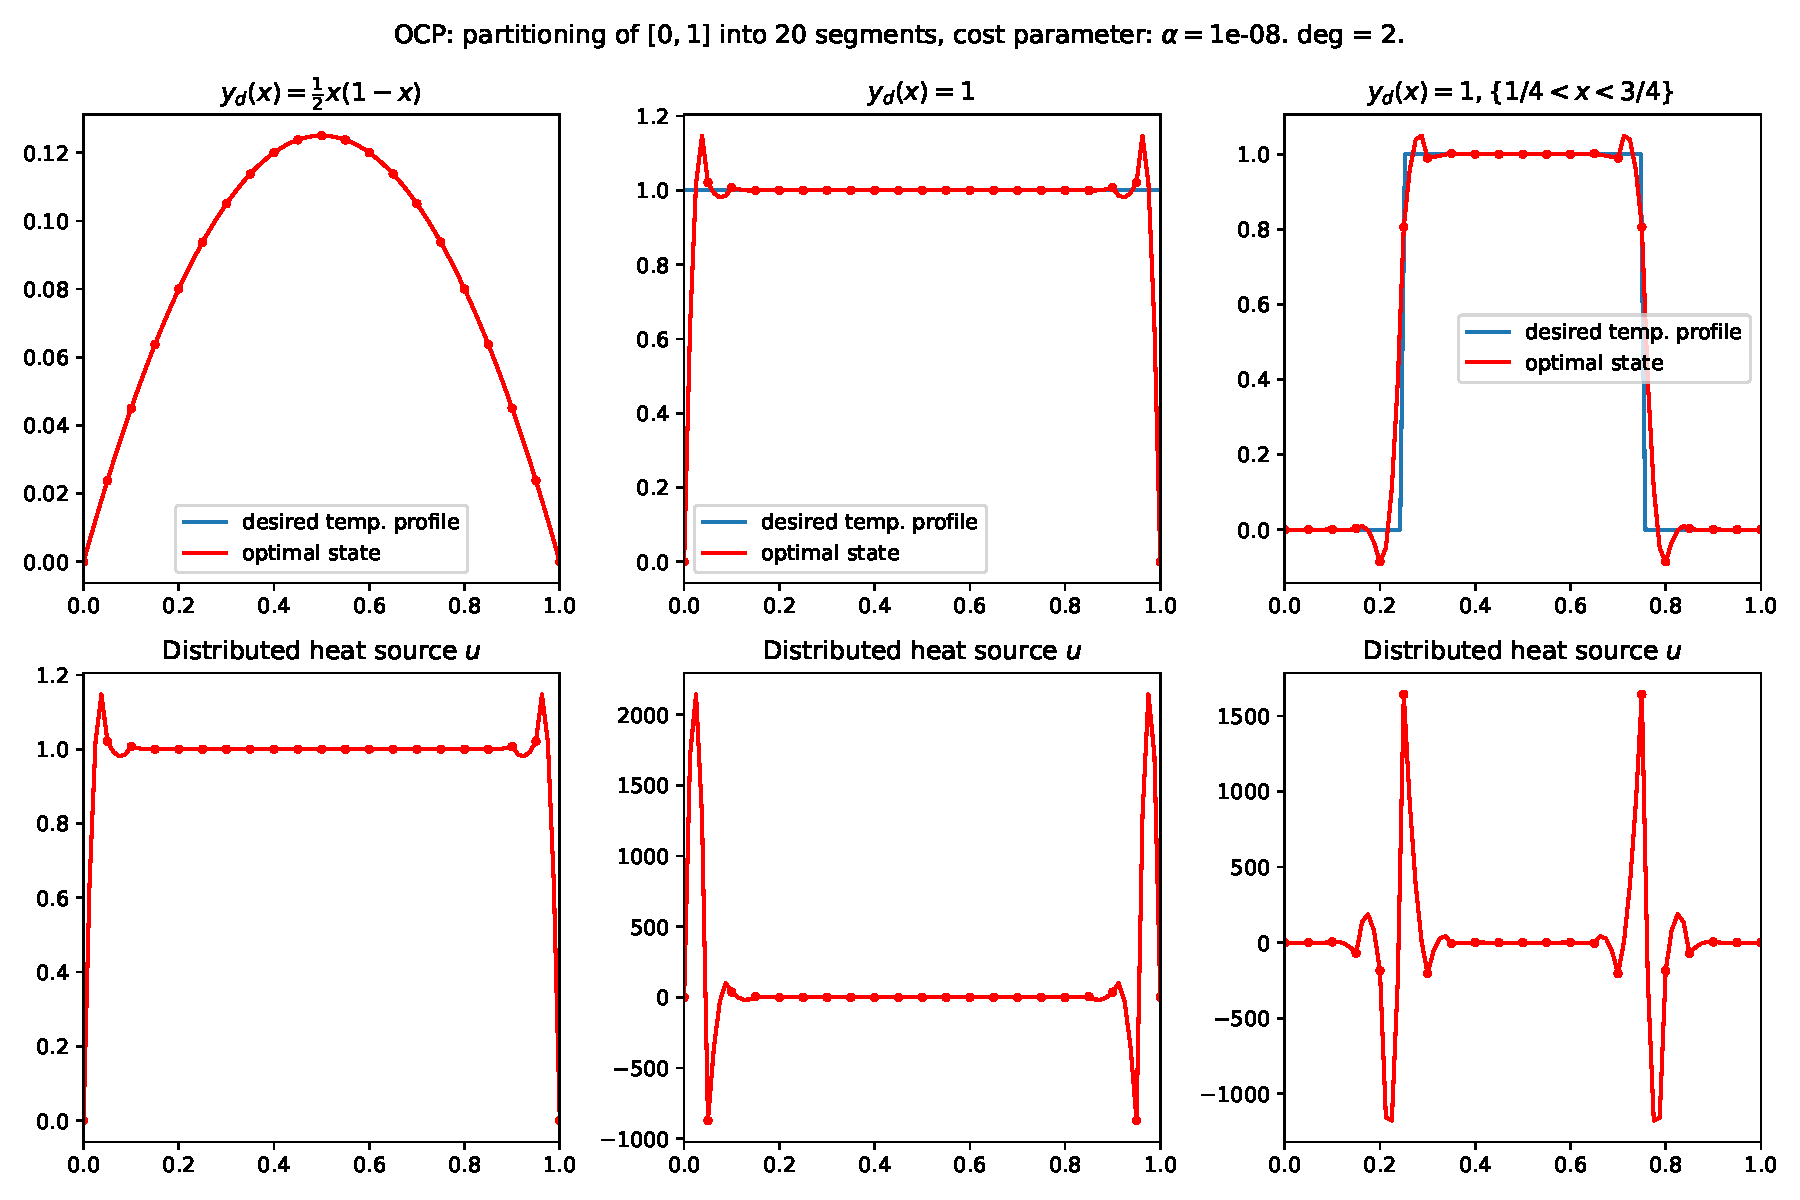
\includegraphics[width=\textwidth]{Images/plots/task2_fig_2.pdf}
  \caption{An optimized control problem for various
    desired temperature profiles. The upper row plots the
    desired temperature profiles and the corresponding 
    optimal state. The lower row plots the
    optimal state for the corresponding problem.
    The cost parameter, $\alpha$, is set to low value.
    To find the optimal state and the optimal control we 
    have partitioned the interval into \( 20 \) elements.
    A second degree Lagrange finite element space has been used.}
  \label{fig:2}
\end{figure}


